\chapter{Linee elettriche: conduttori nudi e cavi}
Nello studio dei sistemi elettrici per l'energia, le linee elettriche costituiscono l'infrastruttura fondamentale preposta alla trasmissione e alla distribuzione dell'energia elettrica tra i centri di produzione e i bacini di carico. Sotto il profilo costruttivo e tecnologico, le linee si suddividono in due categorie fondamentali:
\begin{itemize}
    \item \textbf{Linee con conduttori nudi} $\rightarrow$ impiegate per la trasmissione e la distribuzione aerea, in cui i conduttori sono sospesi nell'aria che funge da principale mezzo dielettrico.
    \item \textbf{Linee in cavo} $\rightarrow$ impiegate per la trasmissione e la distribuzione sotterranea, sottomarina e in specifici contesti aerei, in cui i conduttori sono racchiusi entro un isolante solido o fluido continuo e protetti da involucri esterni.
\end{itemize}

\section{Linee aeree con conduttori nudi}
Le linee aeree con conduttori nudi sono costituite da tre componenti strutturali fondamentali:
\begin{itemize}
    \item \textbf{Conduttori di potenza} $\rightarrow$ elementi metallici tesati nell'aria aventi il compito di convogliare le correnti e trasferire la potenza elettrica attiva e reattiva.
    \item \textbf{Isolatori} $\rightarrow$ elementi preposti a collegare i conduttori di potenza alla struttura di sostegno e ad assicurare l'isolamento elettrico tra le parti in tensione e la struttura che si trova a potenziale di terra.
    \item \textbf{Sostegni} $\rightarrow$ strutture verticali aventi la funzione di sostenere isolatori e conduttori di potenza, garantendo il rispetto delle distanze minime di sicurezza rispetto al suolo e agli ostacoli.
\end{itemize}

Oltre ai conduttori di potenza, sulle linee aeree sono frequentemente installati altri conduttori denominati \textbf{funi di guardia}, posizionati sulla sommità dei sostegni per proteggere la linea dalle sovratensioni di origine atmosferica.
\begin{figure}[H]
	\centering
	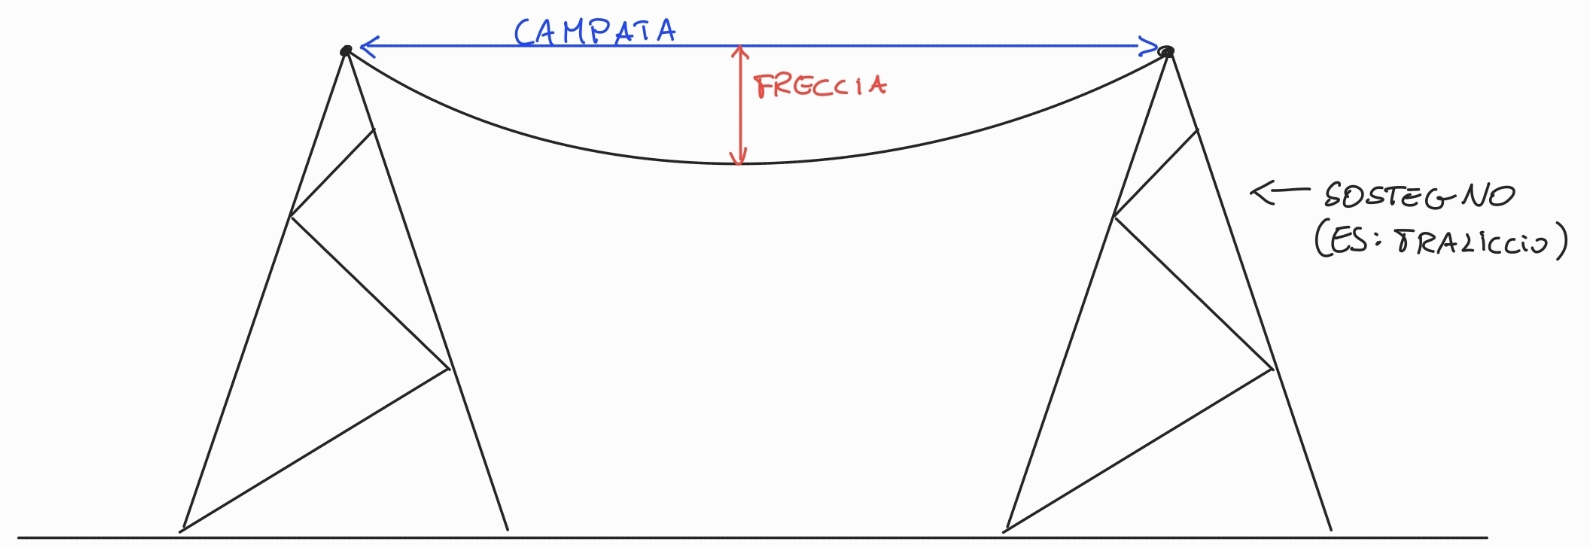
\includegraphics[width=0.7\linewidth]{immagini/linee1}
\end{figure}

\subsection{Conduttori di potenza per linee aeree}
La selezione dei materiali per i conduttori di potenza risponde a requisiti congiunti di conducibilità elettrica, resistenza meccanica alle sollecitazioni esterne, peso specifico e durabilità chimico-ambientale.

I materiali impiegati per i conduttori di potenza comprendono:
\begin{itemize}
    \item \textbf{Rame} $\rightarrow$ impiegato essenzialmente nel campo della bassa tensione. Viene utilizzato sotto forma di filo unico pieno per sezioni inferiori a $10\text{ mm}^2$, oppure sotto forma di corda per sezioni superiori; la corda conferisce una maggiore flessibilità al conduttore, facilitando le operazioni di stendimento e montaggio lungo la tratta.
    \item \textbf{Alluminio} $\rightarrow$ impiegato prevalentemente nel campo della media tensione. Presenta costi di produzione sensibilmente inferiori rispetto al rame e viene adoperato esclusivamente come conduttore cordato a $7$, $19$, $37$ o $61$ fili elementari, stante la difficoltà tecnologica di trafilare fili pieni massicci dotati di sufficiente omogeneità strutturale. L'alluminio possiede una spiccata resistenza agli agenti atmosferici grazie alla formazione spontanea di una sottile pellicola superficiale di ossido (allumina) che ne preserva la matrice metallica.
    \item \textbf{Conduttori bimetallici (Alluminio-Acciaio)} $\rightarrow$ impiegati nelle reti in alta e altissima tensione. Sono realizzati mediante un nucleo interno formato da fili di acciaio zincati e cordati, attorno al quale sono disposti concentricamente fili di alluminio trafilati e cordati. L'acciaio svolge la funzione prevalente di supporto alle sollecitazioni meccaniche di trazione, mentre l'alluminio assicura la conducibilità elettrica della fase; i fili di alluminio sono disposti all'esterno per incrementare il diametro geometrico esterno del conduttore e perché l'alluminio offre una resistenza superiore all'azione corrosiva degli agenti atmosferici. Le proprietà elettromeccaniche del conduttore possono essere calibrate variando il rapporto tra il numero e la sezione dei fili dei due materiali.
    \item \textbf{Lega di alluminio} $\rightarrow$ impiegata nelle linee ad alta tensione; combina le proprietà elettriche tipiche dell'alluminio con una resistenza alle sollecitazioni meccaniche nettamente superiore rispetto al metallo puro.
    \item \textbf{Conduttori a fascio} $\rightarrow$ adottati nelle linee ad altissima tensione (AAT); ciascuna fase della terna trifase è costituita da due o più conduttori in alluminio-acciaio collegati in parallelo e mantenuti a distanza prefissata mediante appositi distanziatori.
\end{itemize}

Le proprietà fisiche, elettriche e meccaniche di riferimento per il rame e per l'alluminio alla temperatura di $20^\circ\text{C}$ sono riassunte nella tabella seguente:

\begin{center}
\begin{tabular}{|l|c|c|}
\hline
\textbf{Caratteristica} & \textbf{Rame} & \textbf{Alluminio} \\
\hline
Resistività elettrica $\rho$ [$\Omega\cdot\text{m}$] & $1{,}7241 \cdot 10^{-8}$ & $2{,}8264 \cdot 10^{-8}$ \\
Sollecitazione a rottura $\sigma_r$ [$\text{MPa}$] & $200 \div 250$ & $120 \div 180$ \\
Densità $\delta$ [$\text{kg}/\text{dm}^3$] & $8{,}89$ & $2{,}70$ \\
Coefficiente di dilatazione lineare $\alpha$ [$\text{K}^{-1}$] & $17 \cdot 10^{-6}$ & $23 \cdot 10^{-6}$ \\
\hline
\end{tabular}
\end{center}

Il confronto quantitativo tra alluminio e rame evidenzia i seguenti aspetti:
\begin{itemize}
    \item Il peso specifico dell'alluminio è pari a circa il $30\%$ di quello del rame.
    \item La resistività elettrica dell'alluminio è superiore di circa il $60\%$ rispetto a quella del rame (ossia una conducibilità elettrica pari a circa il $60\%$).
    \item La resistenza alla rottura dell'alluminio è inferiore rispetto a quella del rame.
    \item Il coefficiente di dilatazione termica dell'alluminio è maggiore, determinando frecce più elevate a parità di distanza tra sostegni successivi (campata).
\end{itemize}

A parità di volume di materiale, una tratta in alluminio peserebbe circa un terzo rispetto a una tratta in rame. Tuttavia, nel dimensionamento elettrico il confronto deve essere condotto a parità di perdite dissipative per effetto Joule, ossia imponendo l'uguaglianza delle resistenze elettriche delle due linee:
\[R = \rho \frac{L}{S}\]
Imponendo $R_{\text{Al}} = R_{\text{Cu}}$ per una medesima lunghezza di linea $L$:
\[\frac{\rho_{\text{Al}}}{S_{\text{Al}}} = \frac{\rho_{\text{Cu}}}{S_{\text{Cu}}} \implies S_{\text{Al}} = \frac{\rho_{\text{Al}}}{\rho_{\text{Cu}}} S_{\text{Cu}} \approx \frac{2{,}8264 \cdot 10^{-8}}{1{,}7241 \cdot 10^{-8}} S_{\text{Cu}} \approx 1{,}64 \, S_{\text{Cu}}\]
Per ottenere la medesima resistenza del conduttore in rame occorre adottare una sezione di alluminio maggiorata di circa il $64\%$. Il rapporto tra le masse dei conduttori a parità di perdite risulta:
\[\frac{M_{\text{Al}}}{M_{\text{Cu}}} = \frac{\delta_{\text{Al}} S_{\text{Al}} L}{\delta_{\text{Cu}} S_{\text{Cu}} L} = \frac{\delta_{\text{Al}}}{\delta_{\text{Cu}}} \frac{\rho_{\text{Al}}}{\rho_{\text{Cu}}} \approx \frac{2{,}70}{8{,}89} \cdot 1{,}64 \approx 0{,}304 \cdot 1{,}64 \approx 0{,}50\]
Di conseguenza, una linea in alluminio a parità di perdite pesa circa il $50\%$ di una equivalente linea in rame, e non il $30\%$ ricavabile dal solo rapporto tra i pesi specifici.

L'impiego dei conduttori bimetallici alluminio-acciaio o in lega di alluminio presenta precisi vantaggi:
\begin{itemize}
    \item La resistenza meccanica totale del conduttore risulta nettamente maggiore.
    \item A parità di lunghezza di campata, il conduttore presenta frecce massime inferiori.
    \item Il diametro esterno risulta maggiore a parità di sezione utile di alluminio.
\end{itemize}

A fronte di tali vantaggi sussistono i seguenti oneri tecnico-progettuali:
\begin{itemize}
    \item Maggiore delicatezza superficiale del materiale conduttore.
    \item Minore peso del conduttore associato al maggior diametro, che determina una maggiore suscettibilità all'azione trasversale del vento; ciò impone una maggiore lunghezza da assegnare alle mensole dei sostegni per mantenere la distanza minima ammissibile di isolamento rispetto alla struttura metallica durante l'oscillazione dei conduttori.
    \item Difficoltà di montaggio legata alla ridotta durezza dell'alluminio (materiale tenero).
    \item Facilità di fusione dei trefoli in alluminio in caso di innesco di archi elettrici, che impone l'adozione di maggiori distanze di sicurezza tra i conduttori di fase.
\end{itemize}

\subsection{Funi di guardia}
Le funi di guardia sono conduttori posti sulla sommità dei sostegni, al di sopra dei conduttori di potenza, con il compito di intercettare le scariche atmosferiche dirette e schermare i conduttori di fase sottostanti, riducendo l'entità delle sovratensioni trasmesse alla linea.

Le funi di guardia moderne sono realizzate mediante corde preformate in acciaio ad alta resistenza. I singoli fili elementari della corda subiscono opportune deformazioni plastiche durante la lavorazione industriale che ne annullano la tendenza naturale allo svolgimento in caso di sollecitazione o taglio; in caso di rottura di un filo, viene impedito che esso si svolga e possa ricadere verso il basso, scongiurando il pericolo di contatto con i conduttori di potenza sottostanti.

\subsection{Isolatori per linee aeree}
Gli isolatori svolgono la funzione congiunta di vincolare i conduttori di fase al sostegno e di assicurare l'isolamento elettrico tra elementi posti a potenziale differente (il conduttore in tensione e la struttura del sostegno collegata a terra).

L'isolatore è costituito da un nucleo in materiale dielettrico e da elementi metallici di aggancio. Il nucleo isolante è sottoposto alla differenza di potenziale determinata dalla tensione nominale di esercizio della linea o dalle eventuali sovratensioni di origine interna o atmosferica.

In condizioni di funzionamento normale, sotto l'azione della differenza di potenziale applicata, l'isolatore è interessato da tre componenti di corrente:
\begin{itemize}
    \item \textbf{Corrente di spostamento} $\rightarrow$ corrente dielettrica alternata legata alla capacità propria dell'isolatore (conduttori separati da dielettrico = capacità).
    \item \textbf{Corrente di conduzione attraverso il nucleo} $\rightarrow$ corrente ohmica derivante dalla resistività volumica finita del materiale dielettrico.
    \item \textbf{Corrente di conduzione superficiale} $\rightarrow$ corrente ohmica che si propaga lungo la superficie esterna dell'isolatore, fortemente incrementata dalla presenza di depositi inquinanti.
\end{itemize}
Il comportamento in funzionamento normale viene modellato \textbf{mediante un circuito equivalente} costituito da tre rami posti in parallelo: un ramo capacitivo (rappresentativo della corrente di spostamento), un ramo resistivo (rappresentativo della conduzione interna nel nucleo dielettrico) e un ulteriore ramo resistivo (rappresentativo della dispersione superficiale).
\begin{figure}[H]
	\centering
	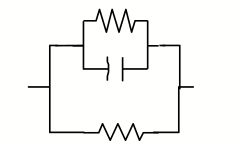
\includegraphics[width=0.25\linewidth]{immagini/linee2}
\end{figure}

Nelle condizioni di funzionamento anormale (innescate da sovratensioni elevate o da grave degrado dielettrico), le correnti che possono manifestarsi sono:
\begin{itemize}
    \item \textbf{Corrente di scarica attraverso il nucleo isolante};
    \item \textbf{Corrente di scarica superficiale}.
\end{itemize}
La geometria dell'isolatore (provvista di nervature e alette a campana per allungare il cammino superficiale della linea di fuga) e la scelta del materiale isolante vengono definite per ridurre al minimo la probabilità che si verifichino tali correnti di scarica.

I requisiti fondamentali che un materiale per isolatori deve possedere sono:
\begin{itemize}
    \item \textbf{Rigidità dielettrica} $\rightarrow$ idoneo valore di tensione sopportabile per unità di spessore prima che si verifichi la perforazione del dielettrico (rottura disruptive o \textit{breakdown}).
    \item \textbf{Resistenza meccanica} $\rightarrow$ adeguati valori di resistenza a trazione, compressione e flessione per sopportare il peso proprio dei conduttori, l'azione del vento e il carico di ghiaccio.
    \item \textbf{Resistenza alla dilatazione termica} $\rightarrow$ stabilità e resistenza alle escursioni termiche ambientali repentine.
\end{itemize}

I materiali impiegati per la realizzazione del nucleo isolante sono la porcellana, il vetro e, nelle realizzazioni più recenti, i materiali compositi:
\begin{itemize}
    \item \textbf{Porcellana} $\rightarrow$ materiale ampiamente impiegato nell'alta tensione; le sue caratteristiche vengono calibrate dosando i materiali costituenti primari: quarzo, caolino e feldspato. La superficie esterna della porcellana viene rivestita con uno strato di smalto vetroso per migliorarne lo stato superficiale (riduzione della rugosità e dell'adesione dello sporco) e regolarizzare le dilatazioni termiche. La porcellana presenta un ottimo comportamento a compressione e un pessimo comportamento a trazione.
    \item \textbf{Vetro temprato} $\rightarrow$ attraverso il trattamento termico di \textit{tempra} si conferisce al vetro una resistenza a trazione da $5$ a $6$ volte superiore rispetto a quella del vetro ricotto, associata a una migliore tenuta alle brusche variazioni di temperatura. In caso di rottura, il vetro temprato si frantuma in piccoli frammenti, facilitando l'individuazione visiva dell'isolatore guasto lungo la linea.
\end{itemize}

I parametri dielettrici, meccanici e termici dei principali materiali isolanti sono riportati nella seguente tabella:

\begin{center}
\begin{tabular}{|l|c|c|c|}
\hline
\textbf{Caratteristica} & \textbf{Porcellana} & \textbf{Vetro Ricotto} & \textbf{Vetro Temprato} \\
\hline
Permittività relativa $\varepsilon_r$ ($20^\circ\text{C}$ e $50\text{ Hz}$) & $6$ & $7{,}5$ & $7{,}5$ \\
Rigidità dielettrica [$\text{kV/m}$] & $170$ & $230$ & $230$ \\
Densità [$\text{kg/dm}^3$] & $2{,}4$ & $2{,}5$ & $2{,}5$ \\
Sollecitazione a rottura [$\text{MPa}$] & $30$ & $20$ & $150$ \\
Modulo di elasticità [$\text{MPa}$] & $77000$ & $74000$ & $72000$ \\
Coefficiente di dilatazione lineare $\alpha$ [$\text{K}^{-1}$] & $5{,}5 \cdot 10^{-6}$ & $9 \cdot 10^{-6}$ & $9{,}1 \cdot 10^{-6}$ \\
\hline
\end{tabular}
\end{center}

Sotto il profilo costruttivo e funzionale, gli isolatori si distinguono in due categorie:
\begin{itemize}
    \item \textbf{Isolatori rigidi} $\rightarrow$ presentano come campo di applicazione limite quello della media tensione.
    \item \textbf{Isolatori sospesi} $\rightarrow$ impiegati per le tensioni superiori alla MT (alta ed altissima tensione).
\end{itemize}

Gli isolatori rigidi sono a loro volta suddivisi in due classi:
\begin{itemize}
    \item \textbf{Isolatori rigidi per tensioni fino a $1\text{ kV}$} $\rightarrow$ costituiti da un unico pezzo di materiale isolante a forma di campana; nella parte sommitale sono presenti apposite scanalature sagomate che servono per l'ammorsamento e il fissaggio del conduttore.
    \begin{figure}[H]
    	\centering
    	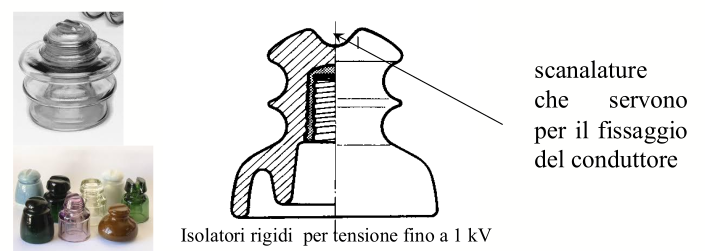
\includegraphics[width=0.55\linewidth]{immagini/linee3}
    \end{figure}
    \item \textbf{Isolatori rigidi per tensioni superiori a $1\text{ kV}$} $\rightarrow$ costituiti da più pezzi di materiale isolante a campana sovrapposti e cementati tra loro mediante materiale legante (cemento).
    \begin{figure}[H]
    	\centering
    	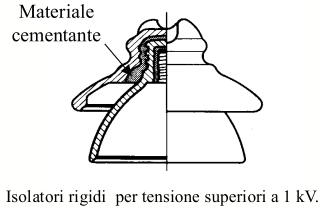
\includegraphics[width=0.35\linewidth]{immagini/linee4}
    \end{figure}
\end{itemize}
L'impiego degli isolatori rigidi è limitato alla media tensione per motivi dimensionali e fisici: al crescere della tensione di esercizio aumentano le distanze di isolamento da garantire in aria e nel dielettrico solido; ciò comporta un aumento proibitivo del volume di materiale isolante necessario, del peso e della probabilità di insorgenza di bolle o imperfezioni interne durante il processo di cottura o colata, che favorirebbero scariche disruptive interne indesiderate.
\begin{figure}[H]
	\centering
	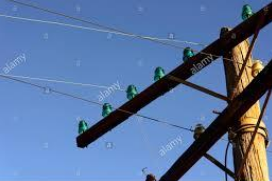
\includegraphics[width=0.3\linewidth]{immagini/linee5}
\end{figure}

Per tensioni superiori alla media tensione si impiegano gli isolatori sospesi, in particolare gli isolatori a \textbf{cappa e perno}:
\begin{figure}[H]
	\centering
	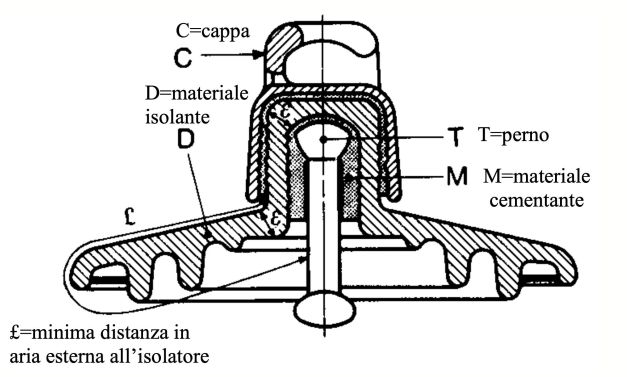
\includegraphics[width=0.4\linewidth]{immagini/linee6}
\end{figure}
\begin{itemize}
    \item \textbf{Cappa metallica (C)} $\rightarrow$ posizionata superiormente all'isolatore; si collega alla mensola del sostegno o al perno dell'isolatore sovrastante.
    \item \textbf{Perno metallico (T)} $\rightarrow$ inserito inferiormente; si aggancia al conduttore di fase o alla cappa dell'isolatore sottostante.
    \item \textbf{Materiale isolante (D)} $\rightarrow$ pezzo unico dielettrico sagomato a calotta interposto tra cappa e perno, avente dimensioni e spessori contenuti.
    \item \textbf{Materiale cementante (M)} $\rightarrow$ malta ad alta adesione che blocca rigidamente il perno e la cappa al corpo dielettrico.
    \item \textbf{Linea di fuga ($\mathcal{L}$)} $\rightarrow$ minima distanza percorsa in aria lungo la superficie sagomata esterna dell'isolatore tra le armature a potenziale differente.
\end{itemize}

Negli isolatori a cappa e perno il collegamento meccanico tra gli elementi avviene mediante snodo a rotula ($R$) con passo definito ($p$):
\begin{figure}[H]
	\centering
	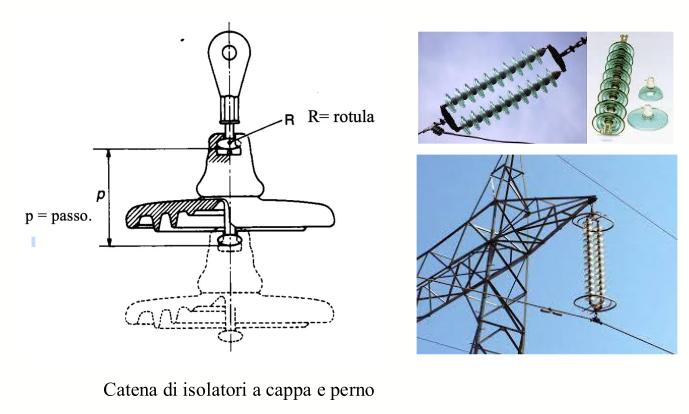
\includegraphics[width=0.7\linewidth]{immagini/linee7}
\end{figure}
Con questa soluzione si superano i vincoli tecnologici degli isolatori rigidi: per isolare linee a tensione crescente non è necessario incrementare le dimensioni del singolo isolatore, ma è sufficiente disporre più isolatori modulari in serie meccanica ed elettrica formando una \textbf{catena di isolatori}. La tenuta dielettrica per linee operanti a livelli di tensione differenti viene così ottenuta semplicemente variando il numero di elementi disposti in catena.

Lungo una catena di isolatori a cappa e perno la distribuzione della tensione presenta andamenti differenziati in base al circuito equivalente adottato:
\begin{itemize}
    \item \textbf{Catena ideale (senza considerare le capacità parassite)} $\rightarrow$ ciascun elemento possiede una capacità propria $C_i$. In assenza di accoppiamenti capacitivi esterni, la corrente capacitiva che fluisce attraverso la catena è la medesima in ciascun isolatore; di conseguenza, la caduta di tensione su ciascun elemento è costante e la tensione si ripartisce in modo rigorosamente lineare tra il sostegno (a potenziale nullo) e il conduttore (a potenziale di fase).
    \item \textbf{Catena reale (considerando le capacità parassite)} $\rightarrow$ entrano in gioco le capacità parassite tra ciascun elemento metallico intermedio e la struttura del sostegno a terra ($C_{is}$), nonché le capacità parassite tra gli elementi e il conduttore di fase in tensione ($C_{ic}$). Le capacità verso terra $C_{is}$ sottraggono frazioni di corrente capacitiva lungo la catena; la corrente che attraversa le capacità proprie $C_i$ risulta progressivamente crescente scendendo dal sostegno verso il conduttore di linea. Di conseguenza, la ripartizione della tensione non è lineare: la frazione di tensione più elevata grava sugli isolatori più vicini al conduttore di potenza, che risultano i più sollecitati elettricamente.
\end{itemize}
\begin{figure}[H]
	\centering
	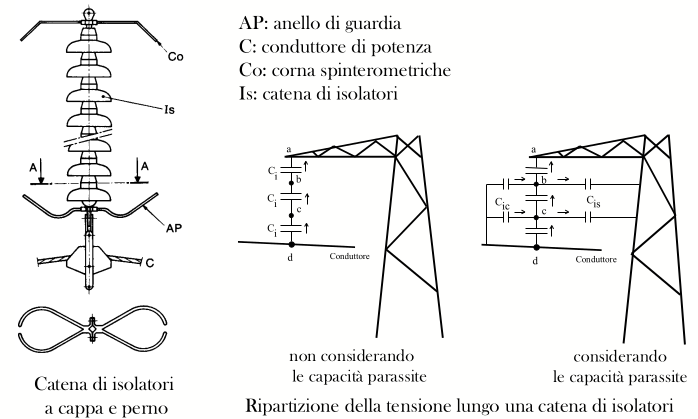
\includegraphics[width=0.8\linewidth]{immagini/linee8}
\end{figure}
Per proteggere la catena e uniformare il campo elettrico si applicano accessori metallici dedicati:
\begin{itemize}
    \item \textbf{Corna spinterometriche (Co)} $\rightarrow$ elettrodi metallici fissati alle due estremità della catena; delimitano una distanza di scarica calibrata in aria inferiore a quella della catena, in modo che eventuali sovratensioni diano origine a una scarica in aria aperta tra le corna, allontanando l'arco dalla superficie del dielettrico ed evitando il danneggiamento termico della catena.
    \item \textbf{Anello di guardia (AP)} $\rightarrow$ conduttore metallico sagomato a forma toroidale od ovale montato all'estremità inferiore della catena in prossimità del conduttore di potenza; incrementa artificialmente le capacità parassite verso il conduttore ($C_{ic}$) compensando l'effetto di $C_{is}$, linearizzando la distribuzione della tensione lungo la catena e riducendo la sollecitazione dielettrica sugli elementi inferiori.
\end{itemize}

\subsection{Sostegni per linee aeree}
I sostegni hanno la funzione di sostenere meccanicamente gli isolatori, i conduttori di potenza e le funi di guardia, mantenendoli alle prescritte distanze reciproche e dal suolo.

I sostegni si classificano in base ai materiali costruttivi impiegati:
\begin{itemize}
    \item \textbf{Sostegni in legno} $\rightarrow$ adoperati molto raramente nelle reti moderne, essenzialmente per linee minori a bassa e media tensione. Sono costituiti da pali ad asse rettilineo ricavati da tronchi di abete o castagno opportunamente trattati con sostanze preservative per ritardare il deperimento biologico; possono essere direttamente infissi nel terreno o ancorati a blocchetti di fondazione in calcestruzzo.
    \begin{figure}[H]
    	\centering
    	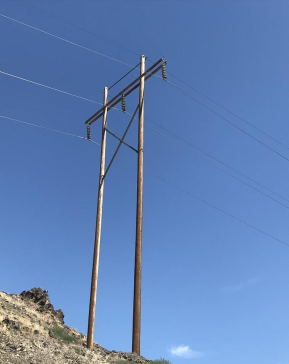
\includegraphics[width=0.3\linewidth]{immagini/linee9}
    \end{figure}
    
    \item \textbf{Sostegni in acciaio} $\rightarrow$ impiegati nell'intero spettro delle tensioni:
    \begin{itemize}
        \item Bassa e media tensione: si utilizzano pali tubolari ad asse rettilineo realizzati mediante tubi di acciaio senza saldatura (tipo Mannesmann).
        \item Alta ed altissima tensione: si impiegano i sostegni a traliccio, formati dall'assemblaggio reticolare di profilati angolari modulari in acciaio zincato collegati mediante bulloni o saldature.
    \end{itemize}
    \item \textbf{Sostegni in cemento armato} $\rightarrow$ costituiti da pali in cemento armato centrifugato a sezione trasversale anulare cava; la parete anulare è attraversata longitudinalmente da armature metalliche formate da tondini di acciaio e riempita con conglomerato cementizio ad alta resistenza.
    \item \textbf{Sostegni in vetroresina} $\rightarrow$ realizzati con materiali compositi a matrice di resine poliestere insature termoindurenti rinforzate con fibre di vetro.
\end{itemize}

I sostegni a traliccio in acciaio per linee ad alta ed altissima tensione presentano diverse configurazioni geometriche:
\begin{itemize}
    \item \textbf{Disposizione tronco-piramidale} $\rightarrow$ fusto reticolare rastremato verso l'alto (costituito da montanti longitudinali e intralicciature diagonali) provvisto di mensole a sbalzo. Le mensole disposte sul medesimo lato del sostegno presentano lunghezze differenti in modo che i conduttori delle fasi ad esse sospese non si trovino allineati sul medesimo piano verticale. Questa asimmetria previene il rischio di corto circuito da "colpo di frusta": durante la stagione invernale i conduttori possono essere appesantiti da manicotti di ghiaccio; in presenza di raffiche di vento, l'eventuale distacco improvviso del manicotto di ghiaccio dal conduttore inferiore ne provoca una repentina risalita elastica verso l'alto (colpo di frusta), che determinerebbe il contatto o l'innesco di arco con il conduttore superiore qualora i due fili fossero disposti sulla medesima verticale.
    \begin{figure}[H]
    	\centering
    	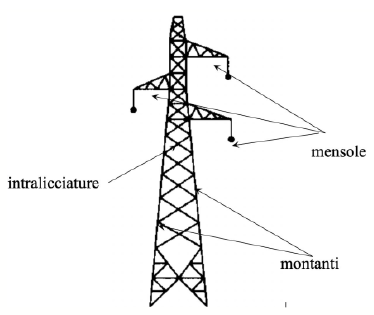
\includegraphics[width=0.4\linewidth]{immagini/linee11}
    \end{figure}
    \item \textbf{Disposizione a portale} $\rightarrow$ struttura costituita da due piedritti verticali reticolari uniti superiormente da una traversa orizzontale; i tre conduttori di fase sono disposti complanari al di sotto della traversa, mentre le due funi di guardia sono montate alle due estremità superiori della struttura.
    \begin{figure}[H]
    	\centering
    	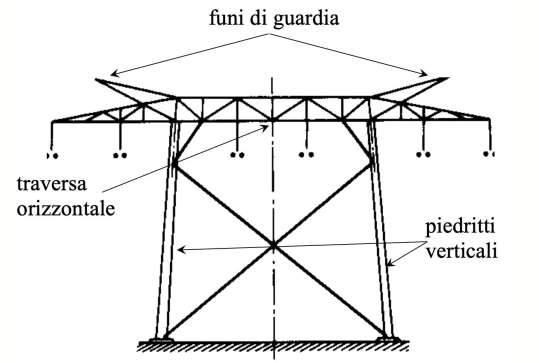
\includegraphics[width=0.4\linewidth]{immagini/linee12}
    \end{figure}
    \item \textbf{Disposizione ad Y} $\rightarrow$ fusto a base tronco-piramidale rastremata che si allarga nella parte superiore assumendo la forma a calice ad Y, provvisto di traversa orizzontale di supporto dei conduttori e di prolungamenti superiori per l'ancoraggio delle funi di guardia.
    \begin{figure}[H]
    	\centering
    	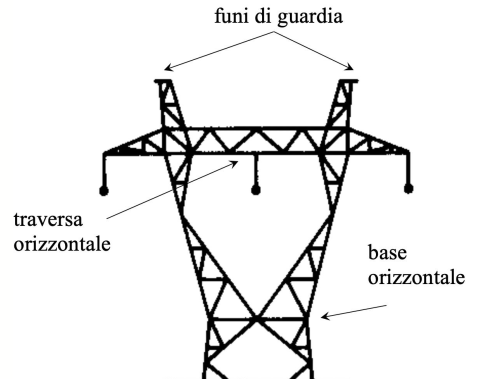
\includegraphics[width=0.4\linewidth]{immagini/linee13}
    \end{figure}
    \item \textbf{Sostegni di design innovativo} $\rightarrow$ strutture progettate per mitigare l'impatto visivo e ambientale, tra cui il sostegno tipo Foster (sviluppato nell'ambito del concorso 2001 per la linea Santa Barbara--Tavarnuzze, realizzato nel 2009) e il sostegno tipo Germoglio (sviluppato nel concorso 2007 per le nuove serie di sostegni per elettrodotti a $380\text{ kV}$).
    \begin{figure}[H]
    	\centering
    	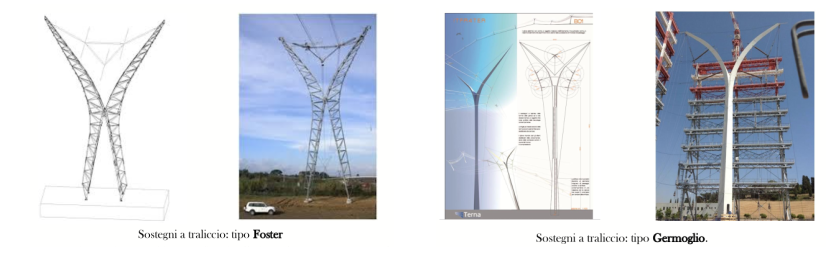
\includegraphics[width=0.9\linewidth]{immagini/linee14}
    \end{figure}
\end{itemize}


I sostegni in vetroresina presentano proprietà fisiche e meccaniche (elevato rapporto resistenza-peso, eccellente tenuta alla corrosione e ingombro limitato) che assicurano precisi vantaggi:
\begin{itemize}
    \item Elevata leggerezza, che si traduce in una marcata riduzione dei costi di trasporto e facilità di installazione in cantiere.
    \item Assenza di deformazioni permanenti qualora la struttura sia sottoposta a sollecitazioni meccaniche prossime al limite di rottura, unita all'assenza di fenomeni vibratori ad alta frequenza indotti dalle correnti d'aria.
    \item Ottima resistenza agli agenti atmosferici e all'azione corrosiva dell'ambiente, con conseguente eliminazione degli oneri di manutenzione ordinaria.
    \item Elevata sicurezza intrinseca rispetto ai pericoli di incendio.
\end{itemize}

\section{Linee in cavo}
Le linee in cavo vengono impiegate per la trasmissione e la distribuzione dell'energia elettrica in posa sotterranea (ambiti urbani ad alta densità o attraversamenti protetti), sottomarina (collegamenti interinsulari e transfrontalieri) e in taluni casi in posa aerea (tramite cavi cordati ad elica autoportanti).

Un impianto di linea in cavo è costituito da due elementi impiantistici:
\begin{itemize}
    \item \textbf{Cavi} $\rightarrow$ condotti elettrici flessibili continui preposti al trasporto della corrente.
    \item \textbf{Accessori di raccordo} $\rightarrow$ comprendono gli \textbf{accessori di estremità} (terminali per il collegamento del cavo a una linea aerea o a un sistema di sbarre di cabina, con gestione del gradiente di potenziale all'interruzione degli schermi) e le \textbf{giunzioni} (manicotti intermedi che assicurano la continuità elettrica, dielettrica e meccanica tra due tratti successivi di cavo su lunghe distanze, rese necessarie dai limiti di fabbricazione e trasporto delle bobine).
\end{itemize}

Il cavo è costituito da tre elementi fondamentali:
\begin{itemize}
    \item \textbf{Conduttori} $\rightarrow$ uno o più conduttori metallici per il transito della corrente di carico.
    \item \textbf{Isolante solido o fluido} $\rightarrow$ mezzo dielettrico continuo che garantisce l'isolamento verso l'esterno e tra le fasi (a differenza delle linee aeree dove l'isolamento è garantito dall'aria).
    \item \textbf{Guaina di protezione} $\rightarrow$ involucro stagno continuo che preserva il cavo da infiltrazioni di umidità, sollecitazioni meccaniche e aggressioni chimiche.
\end{itemize}

Nel cavo possono essere inoltre presenti:
\begin{itemize}
    \item \textbf{Armatura metallica} $\rightarrow$ costituita da nastri di acciaio o fili di acciaio per proteggere il cavo da urti, schiacciamento e trazioni meccaniche durante la posa o l'esercizio.
    \item \textbf{Schermi semiconduttori} $\rightarrow$ nastri o estrusioni a base di mescole caricate con nerofumo, posizionati a contatto dei conduttori per livellarne le irregolarità geometriche superficiali evitando amplificazioni localizzate del campo elettrico (effetto punta).
    \item \textbf{Schermi metallici} $\rightarrow$ realizzati in piombo, rame o alluminio per uniformare le linee del campo elettrico, confinare il campo all'interno del dielettrico e drenare le correnti capacitive e di guasto verso terra.
\end{itemize}

I materiali costitutivi impiegati nelle diverse parti del cavo comprendono:
\begin{itemize}
    \item \textbf{Conduttori}: rame e alluminio, con criteri di scelta che variano in funzione della classe di tensione, degli ingombri di posa e delle perdite ammissibili.
    \item \textbf{Isolanti}: carta impregnata e isolanti polimerici estrusi.
    \item \textbf{Guaine}: piombo, PVC, oppure alluminio (adottato nei cavi con conduttori in alluminio).
\end{itemize}

La carta impiegata nell'isolamento deve essere di pura cellulosa. La rigidità dielettrica della carta secca è modesta (dell'ordine di pochi $\text{kV/mm}$); per acquisire le proprietà isolanti necessarie, la carta viene impregnata con sostanze fluide o viscose. Gli impregnanti più utilizzati sono gli oli minerali o sintetici; associando l'olio a cicli industriali di essiccazione e impregnazione sottovuoto si ottengono isolanti di altissimo livello prestazionale.

Gli isolanti estrusi di impiego industriale comprendono:
\begin{itemize}
    \item \textbf{PVC} $\rightarrow$ policloruro di vinile.
    \item \textbf{PE e derivati} $\rightarrow$ polietilene e polietilene reticolato (XLPE).
    \item \textbf{EPR} $\rightarrow$ gomma etilenpropilenica.
    \item \textbf{Gomma butilica}.
\end{itemize}

La valutazione comparativa tra i diversi materiali isolanti estrusi alle diverse classi di tensione si fonda su tre proprietà dielettriche fondamentali:
\begin{itemize}
    \item \textbf{Rigidità dielettrica} $\rightarrow$ massimo valore di tensione prima del verificarsi della scarica di breakdown.
    \item \textbf{Perdite dielettriche ($\tan\delta$)} $\rightarrow$ grandezza proporzionale all'aliquota di potenza attiva dissipata sotto forma termica nel dielettrico per effetto della tensione alternata applicata.
    \item \textbf{Resistenza alle scariche parziali} $\rightarrow$ parametro indicatore della vita utile e della resistenza al degrado elettrochimico del dielettrico nel tempo.
\end{itemize}

\subsubsection{Perdite dielettriche e fattore di perdita $\tan\delta$}
Il comportamento dielettrico di un materiale isolante sottoposto a una tensione di prova alternata $U_{\text{test}}$ viene modellato considerando l'isolante come una struttura bipolare non ideale, schematizzabile mediante il parallelo tra una capacità ideale $C$ e una resistenza ideale di dispersione $R$.

La corrente complessiva $\bar{I}$ che fluisce nell'isolante è data dalla somma fasoriale di due componenti:
\[\bar{I} = \bar{I}_R + \bar{I}_c\]
dove:
\begin{itemize}
    \item $\bar{I}_R$ indica la corrente resistiva in fase con la tensione $U_{\text{test}}$, imputabile alla conducibilità ohmica residua del dielettrico e alle dissipazioni per polarizzazione.
    \item $\bar{I}_c$ indica la corrente capacitiva ideale in quadratura di anticipo ($90^\circ$) rispetto alla tensione $U_{\text{test}}$.
\end{itemize}

Nel piano fasoriale, l'angolo $\varphi$ rappresenta lo sfasamento tra la corrente totale $I$ e la tensione applicata $U_{\text{test}}$. L'angolo $\delta$, denominato \textbf{angolo di perdita dielettrica}, è il complementare di $\varphi$:
\[\delta = 90^\circ - \varphi\]
\begin{figure}[H]
	\centering
	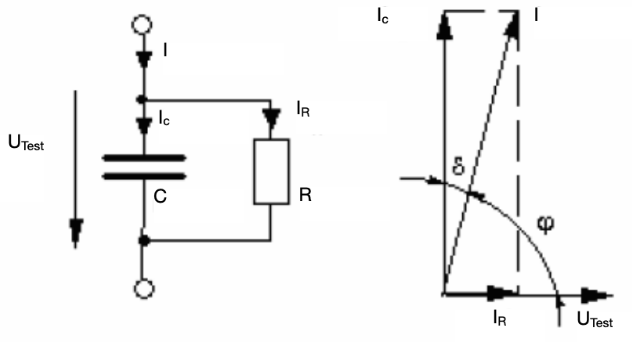
\includegraphics[width=0.45\linewidth]{immagini/linee15}
\end{figure}
La tangente dell'angolo di perdita $\tan\delta$ quantifica il rapporto tra l'aliquota di potenza attiva dissipata $P_r$ e la potenza reattiva generata $Q_c$:
\[\tan\delta = \frac{P_r}{Q_c} = \frac{I_r}{I_c} = \frac{X_c}{R}\]
dove $X_c = \frac{1}{\omega C}$ rappresenta la reattanza capacitiva dell'isolante e $R$ la sua resistenza equivalente.

Ai fini dell'efficienza e della tenuta dielettrica, si richiede la minima potenza attiva dissipata possibile nel mezzo: a parità di tensione di prova $U_{\text{test}}$, un valore di $\tan\delta$ più basso è indice di una qualità dielettrica superiore del materiale isolante, corrispondendo a minori perdite dissipative $P_r$.

\section{Tipologie costruttive dei cavi}

\subsection{Cavi in Carta Impregnata}
Il ciclo industriale di fabbricazione di un cavo in carta impregnata si articola in tre fasi:
\begin{enumerate}
    \item \textbf{Nastratura} $\rightarrow$ il conduttore metallico viene avvolto a spirale con strati successivi di nastri di carta pura (a spessore costante o crescente) fino a raggiungere lo spessore isolante prescritto dal livello di tensione, costituendo l'\textbf{anima} del cavo. Nel cavo unipolare la nastratura della carta termina qui. Nel cavo tripolare le tre anime isolate vengono cordate insieme a elica, riempiendo gli interstizi residui con opportuno materiale isolante di riempimento (carta o iuta); attorno alle tre anime cordate viene applicata un'ulteriore nastratura perimetrale di carta denominata \textbf{cintura}.
    \item \textbf{Impregnamento} $\rightarrow$ l'anima (nel caso unipolare) o il fascio delle tre anime fasciate dalla cintura (nel caso tripolare) vengono introdotte all'interno di una vasca a chiusura ermetica; nella vasca viene praticato il vuoto e viene eseguito un processo di essiccamento termico per rimuovere ogni traccia di aria e umidità residua. Successivamente viene immesso l'olio isolante e la vasca viene posta sotto pressione in modo che l'olio penetri all'interno dell'intera massa di carta fino a impregnarla completamente.
    \item \textbf{Applicazione della guaina e armature esterne} $\rightarrow$ il cavo estratto dalla vasca attraversa una macchina per l'estrusione della guaina protettiva metallica continua, generalmente in piombo. All'esterno della guaina di piombo viene applicato uno strato di iuta catramata e un'armatura protettiva esterna costituita da un doppio strato di eliche in nastro di acciaio, con funzioni congiunte di resistenza alle sollecitazioni meccaniche e protezione contro i contatti accidentali.
\end{enumerate}

Nei cavi in carta impregnata la distribuzione dei campi elettromagnetici dà luogo a sollecitazioni differenti in base alla geometria costruttiva:
\begin{itemize}
    \item \textbf{Cavo unipolare}:
    \begin{itemize}
        \item Sollecitazione da campo elettrico $\rightarrow$ per ragioni di simmetria assiale, le linee del campo elettrico si sviluppano in direzione rigorosamente radiale dal conduttore verso lo schermo esterno, mentre le superfici equipotenziali costituiscono cilindri concentrici coassiali al conduttore. La carta impregnata risulta sollecitata punto per punto in direzione normale alla giacitura dei nastri, condizione in cui il dielettrico manifesta la massima rigidità dielettrica.
        \item Sollecitazione da campo magnetico $\rightarrow$ la corrente alternata che fluisce nel singolo conduttore genera un campo magnetico concatenato variabile che induce correnti parassite dissipative nella guaina metallica di piombo e nell'armatura di acciaio. Per limitare tali correnti e le relative perdite, attorno all'anima vengono disposti due nastri di acciaio avvolti in verso opposto, generando campi magnetici indotti in opposizione di fase che si compensano.
        \item Comportamento complessivo $\rightarrow$ il cavo unipolare possiede un ottimo comportamento nei riguardi del campo elettrostatico, ma un comportamento sfavorevole nei riguardi del campo magnetico; trova applicazioni crescenti all'aumentare della tensione di esercizio.
    \end{itemize}
    
    \newpage
    \item \textbf{Cavo tripolare a cintura (campo non radiale)}:
    \begin{itemize}
        \item Sollecitazione da campo elettrico $\rightarrow$ nelle tre anime fluiscono tensioni sinusoidali sfasate di $120^\circ$. Viene meno la simmetria cilindrica e le linee del campo elettrico interagiscono reciprocamente incurvandosi. Sul dielettrico agiscono componenti del campo elettrico sia normali che tangenziali rispetto agli strati di carta. La carta presenta una modesta rigidità dielettrica lungo la direzione tangenziale di scorrimento tra i nastri; la presenza di tali componenti tangenziali limita la tensione di esercizio di questa configurazione a valori di $20 \div 30\text{ kV}$.
        \item Sollecitazione da campo magnetico $\rightarrow$ il cavo tripolare manifesta un comportamento ideale: in condizioni simmetriche ed equilibrate la somma delle tre correnti istantanee è rigorosamente nulla:
        \[i_1(t) + i_2(t) + i_3(t) = 0\]
        I campi magnetici generati dalle tre correnti sfasate costituiscono a loro volta una terna simmetrica a risultante nulla all'esterno, annullando la circolazione di correnti parassite indotte nei rivestimenti metallici esterni.
    \end{itemize}
    \item \textbf{Cavo tripolare a campo radiale (schermato, $60 \div 70\text{ kV}$)}:
    \begin{itemize}
        \item Per estendere l'impiego del cavo tripolare a tensioni superiori si inserisce attorno a ciascuna anima, al di sopra dell'ultimo strato di carta, un nastro di carta metallizzata prima della cordatura comune.
        \item Il nastro metallizzato vincola le superfici equipotenziali ad assumere la forma di cilindri coassiali a ciascun conduttore, rendendo il campo elettrico puramente radiale all'interno di ogni singola anima.
        \item Le tre anime si comportano elettrostaticamente come tre cavi unipolari indipendenti esenti da componenti tangenziali del campo, preservando al contempo il vantaggio magnetico di somma nulla delle correnti.
    \end{itemize}
\end{itemize}
\begin{figure}[H]
	\centering
	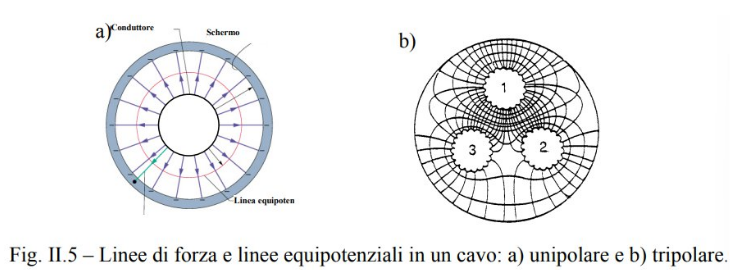
\includegraphics[width=0.8\linewidth]{immagini/linee16}
\end{figure}

\subsection{Cavi ad olio fluido}
Nelle applicazioni ad altissima tensione (fino a $400\text{ kV}$) si adottano i cavi ad olio fluido:
\begin{itemize}
    \item \textbf{Cavo tripolare ad olio fluido a pressione esterna ($15\text{ bar}$)}:
    \begin{itemize}
        \item \textbf{A} $\rightarrow$ anima conduttrice in rame.
        \item \textbf{Is} $\rightarrow$ isolante in carta impregnata.
        \item \textbf{FG} $\rightarrow$ fili di scorrimento metallici disposti a spirale esternamente a ciascuna anima per facilitare le operazioni di traino e infilaggio nel condotto.
        \item \textbf{T} $\rightarrow$ tubo di acciaio rigido continuo entro cui sono alloggiate le tre anime, riempito di olio dielettrico mantenuto alla pressione costante di $15\text{ bar}$.
    \end{itemize}
    \begin{figure}[H]
    	\centering
    	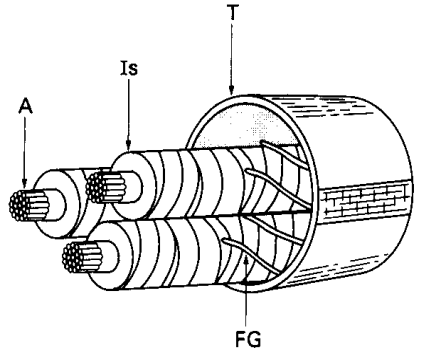
\includegraphics[width=0.35\linewidth]{immagini/linee17}
    \end{figure}
    
    \item \textbf{Cavo ad olio fluido a pressione interna}:
    \begin{itemize}
        \item \textbf{A} $\rightarrow$ spirale interna in acciaio di supporto meccanico.
        \item \textbf{Ca} $\rightarrow$ canale centrale di espansione e circolazione dell'olio isolante.
        \item \textbf{C} $\rightarrow$ conduttore in fili profilati di rame formanti un condotto cilindrico cavo.
        \item \textbf{SC} $\rightarrow$ strati di carta semiconduttrice disposti sia all'interfaccia con il conduttore che all'interfaccia con la guaina per livellare il campo elettrico.
        \item \textbf{Is} $\rightarrow$ isolante primario in carta impregnata.
        \item \textbf{G} $\rightarrow$ guaina di tenuta in piombo.
        \item \textbf{F} $\rightarrow$ nastratura in acciaio con funzione di contenimento meccanico della pressione interna e schermatura del campo magnetico verso l'esterno.
        \item \textbf{GP} $\rightarrow$ guaina protettiva esterna anticorrosiva.
    \end{itemize}
\end{itemize}
\begin{figure}[H]
	\centering
	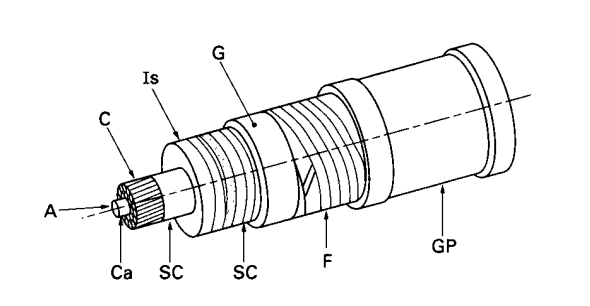
\includegraphics[width=0.55\linewidth]{immagini/linee18}
\end{figure}


\subsection{Cavi in isolante estruso}
Nei moderni impianti di distribuzione e trasmissione si impiegano in prevalenza cavi con dielettrico polimerico estruso, la cui struttura varia in funzione della classe di tensione:
\begin{itemize}
    \item \textbf{Cavo BT (Bassa Tensione)}:
    \begin{itemize}
        \item Conduttore in corda rigida di rame stagnato.
        \item Isolante primario estruso in gomma butilica.
        \item Guaina protettiva esterna in PVC.
    \end{itemize}
    \item \textbf{Cavo MT (Media Tensione)}:
    \begin{itemize}
        \item Conduttore in corda rigida di rame stagnato.
        \item Nastro semiconduttore interno, applicato per livellare le discontinuità superficiali dei trefoli metallici della corda ed evitare amplificazioni di campo dielettrico per effetto punta.
        \item Isolante primario estruso in gomma etilenpropilenica (EPR).
        \item Schermo metallico formato da un nastro di rame avvolto a spirale continua.
        \item Guaina protettiva esterna in PVC.
    \end{itemize}
    \item \textbf{Cavo AT (Alta Tensione)}:
    \begin{itemize}
        \item Conduttore centrale in corda compatta di rame stagnato.
        \item Strato semiconduttore interno continuo.
        \item Isolante primario in gomma etilenpropilenica (EPR) ad alto spessore.
        \item Strato semiconduttore esterno continuo.
        \item Schermatura metallica a treccia formata da fili di rame intrecciati.
        \item Guaina protettiva esterna in PVC.
    \end{itemize}
\end{itemize}
\begin{figure}[H]
	\centering
	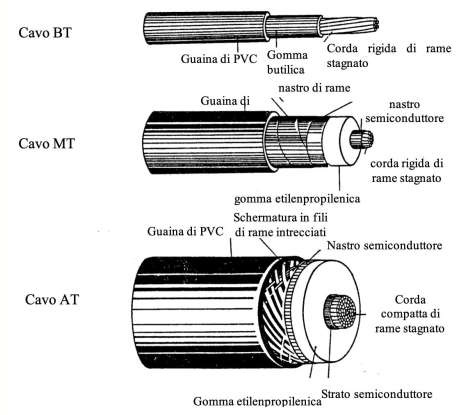
\includegraphics[width=0.6\linewidth]{immagini/linee19}
\end{figure}


\newpage
\section{Designazione normativa dei cavi}
L'identificazione univoca delle caratteristiche costruttive e dielettriche dei cavi di bassa e media tensione è disciplinata dalle tabelle di unificazione normativa.

\subsection{Designazione secondo CEI-UNEL 35011}
\begin{figure}[H]
	\centering
	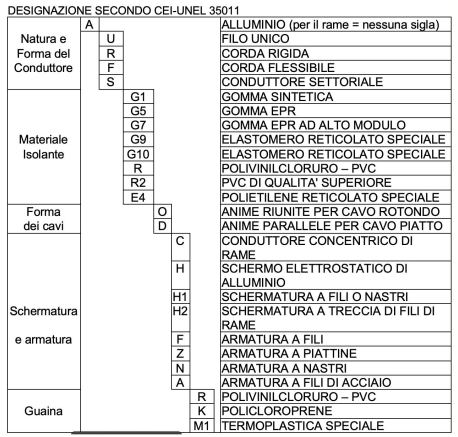
\includegraphics[width=0.6\linewidth]{immagini/linee20}
\end{figure}


\subsection{Designazione armonizzata secondo CEI 20-27}
La norma CEI 20-27 recepisce la codifica unificata europea CENELEC per i cavi isolati di bassa tensione, articolata secondo la seguente sequenza di simboli:
\begin{figure}[H]
	\centering
	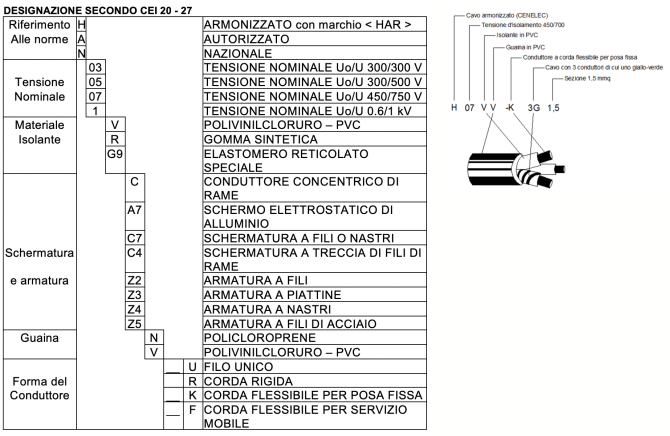
\includegraphics[width=0.9\linewidth]{immagini/linee21}
\end{figure}
